\section{Database}

Med udgangspunkt i \gls{moscow} analysen i afsnit~\pageref{sec:moscow} blev det første udkast til databasen lavet. Meningen var at opfylde punktet: 

\begin{itemize}
	\item Der skal kunne oprettes en bruger til systemet.
\end{itemize}

For at lave dette på en måde som gjorde udvidelse let, kom første udkast til at se ud som vist på figur~\ref{fig:database_class_1}. Adgangen til databasen skulle være simpel. Dette var på grund af grænsefladen til resten af system, som skulle udvikles samtidigt. På denne måde skulle de øvrige grupper ikke ændre deres brug af \textit{ISmartpool} interfacet.  skulle der laves én klasse som ville have associationer til specialiserede klasser. Figur~\ref{fig:database_class_1} viser hvordan kaldet fra \textit{context} går gennem klassen \textit{ISmartpool}

\begin{figure}[h]
	\centering
	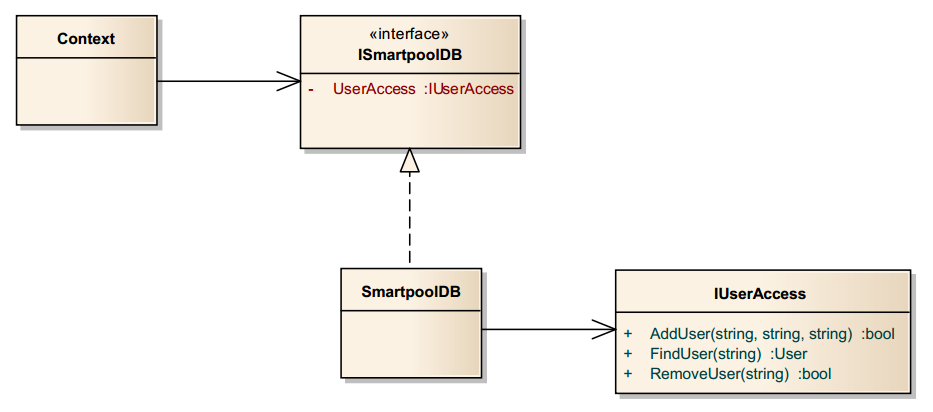
\includegraphics[width=0.9\linewidth]{figs/design/database_class_1}
	\caption{Første design for database-adgang.}
	\label{fig:database_class_1}
\end{figure}

På denne måde skulle \textit{UserAccess} klasse så stå for adgang til brugerinformationer i databasen. 

Der skulle så laves en simple database, med det eneste formål at kunne indeholde disse basale informationer om brugerne af systemet.

\begin{itemize}
	\item Navn (for, mellem og -efternavn)
	\item Email
	\item Kodeord
\end{itemize}

Med \gls{ef} blev følgende model lavet til at opfylde dette krav.

\begin{figure}[h]
	\centering
	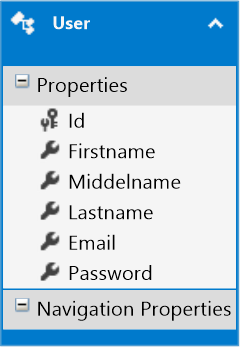
\includegraphics[width=0.25\linewidth]{figs/design/database_model_1}
	\caption{Model for første design for database-adgang.}
	\label{fig:database_model_1}
\end{figure}

Udfra dette blev et script genereret, som så skulle køres mod en localdb. Nu var databasen oprettet og implementeringen af \textit{UserAccess} kunne starte.